% !TeX root = ../document_maitre.tex

\label{imageAnimee}

Dans cette partie, l'indexation semi-automatisée est pensée dans son application à un objet patrimonial particulier : l'\gls{imgani}. Les spécificités de cet objet et sa complexité d'indexation, même humaine, le placent au \coeur des volontés d'automatisation de son indexation et en démontrent les limites.

\subsection{Définition de l'indexation et de l'\gls{imgani} }

L'indexation est une opération d'analyse et d'extraction d'informations contenues par les objets patrimoniaux afin de produire des métadonnées descriptives attribuant des caractéristiques uniques à chaque objet. Pour cela, l'indexation s’appuie sur différents outils comme des \gls{thesaurus} afin d'en faciliter l'exécution et de créer une homogénéité.\footcite[p.2]{directiondesarchivesdefranceNoteDinformationDITN2007} Sa \guillemet{semi-automatisation} est l'idée de pouvoir se reposer partiellement sur des outils \gls{IA} capable de proposer des métadonnées dans les bons champs, respectant les normes et standards. L'opérateur humain n'ayant plus qu'à valider ou modifier ce dernières.

Pour penser de tels processus appliqués à l'\gls{imgani}, il convient d'en comprendre la nature et complexité. La \gls{FIAF} la définit comme un objet regroupant des images enregistrées successivement dont la diffusion donne une impression de mouvement.\footcite[p.5]{fairbairnManuelCatalogageImages} Cela peut être un \gls{rush}, c'est-à-dire l'enregistrement brute, ou bien une version retravaillée en \guillemet{post-production}. Elle peut intégrer des bandes sonores enregistrés au moment de la capture des images ou rajoutées en \guillemet{post-production}. Ainsi, un film, une vidéo, un extrait, une bande-annonce, une publicité sont des \glspl{imgani}.

Elle se caractérise également par sa diversité matérielle. L'\gls{imgani} a d'abord été enregistré sur des bandes au nitrate d'argent photosensible. Puis sur des bandes vidéos magnétiques permettant l'enregistrement sonore en simultané. Puis sur des supports optiques gravés, comme les DVD. Et enfin les supports numériques, tels des clés USB ou des \textit{clouds}, les stockant dans des formats digitaux comme le MP4 le MKV. Ils servent à l'enregistrement original et/ou à la diffusion. Pour le format numérique, on distingue les formats numériques de production des formats numériques de diffusion. Les formats varient en fonction du matériel utilisé pour enregistré et celui utilisé par diffusé. Pour des raisons de conservation on rencontre un principe similaire sur l'\gls{imgani} physique, ce qui fait qu'une même \oe{uvre} existe dans différentes matérialités simultanément ou successivement.\newline %pour l'absence d'un \gls{oe}. Je ne fais pas référence au niveau WEMI donc inaproprié.

Il y a également une notion d'état amené par la \guillemet{post-production}. Prenons un film récent comme \textit{Avatar (2009)} du réalisateur James Cameron. Le film diffusé au public est uniquement fait d'images de synthèse et d'effets spéciaux numériques. Cependant, tout cela a été produit à partir de \glspl{rush} sur lesquels figurent des acteurs, d'autres décors et matériels. Il existe donc deux états du film : la version \guillemet{brute}, composé de \glspl{rush}, et la version diffusée. Ces transformations extrêmes restent rares, cependant la \guillemet{post-production} a tendance à prendre une place grandissante.\newline

L'\gls{imgani} nécessite un matériel de diffusion. En effet, sa projection est un aspect fondamental car c'est ce qui fait apparaître la notion de mouvement. Cela implique la conservation des équipements de diffusion propres à chaque matérialité de l'\gls{imgani}.\footcite{edmondsonPHILOSOPHYPRINCIPLES} Cela demande donc d'entretenir ce matériel précieux, certains équipements n'étant plus fabriqués. Il y a donc une double obsolescence : celle des supports de diffusion et celle de l'objet patrimonial. Ainsi, une \gls{imgani} produite au début du XX\textsuperscript{ème} siècle sur une bande en nitrate d'argent et doublement en danger. D'abord par sa conversation, son composé chimique étant instable et pouvant prendre feu si mal conservé. Ensuite pour sa diffusion, le projecteur n'étant plus fabriqué et les compétences pour l'entretenir se raréfie.\footcite[p.39 et 54]{edmondsonPHILOSOPHYPRINCIPLES}

Il y a également une grande diversité conceptuelle. Nous ne parlons pas de film, de vidéos ou encore de documentaire car ils représentent des réalités différentes leur réalisation, utilisation, objectif, diffusion et conservation. L'\gls{imgani} concerne aussi bien un film amateur que professionnel, et toutes la typologie que cela recouvre, mais aussi les séries, publicités, etc.\footcite[p.5]{fairbairnManuelCatalogageImages}. Chaque typologie possède ses caractéristiques uniques et donc sa propre indexation.\footcite[p.18 et 34]{edmondsonPHILOSOPHYPRINCIPLES}\newline

C'est un objet patrimonial unique, faisant face à ses propres défis non partagés avec les autres objets patrimoniaux. Dès lors, au sein de collections hétérogènes l'indexation de l'\gls{imgani} se doit d'être particulière afin de prendre en compte toutes les complexités brièvement explorées.

\subsection{Le \gls{FRBR} et le \gls{WEMI}}

\label{FRBR-WEMI}

Les prémices de cette gestion particulière apparaissent en 1998. Jusqu'alors, la norme internationale qu'est l'ISBD structurait les données bibliographiques autour du seul objet physique. Cela ne permettait pas de créer du lien au sein des collections internes et externes et l'apparition de déclinaisons, comme l'ISBD(A) pour les livres anciens, a finalement fragilisé l'homogénéité des données. Devant l'évolution des besoins utilisateurs, visant à simplifier les requêtes, l'ISBD s'est révélé peu adapté. Une \oe{uvre} ne pouvant être présentée avec ses déclinaisons successives, ni ses liens avec d'autres \oe{uvres}, la démarche exploratoire de l'utilisateur s'est retrouvé trop limité et frustrante. 

Ainsi, l'\gls{IFLA} souhaite réorganiser la gestion de cet objet patrimonial en déplaçant le point d'intérêt de l'exemplaire vers un ensemble conceptuel plus vaste et structuré. C'est le \coeur du modèle \gls{FRBR} qu'elle publie afin de repenser tout ce système de description et de gestion des données bibliographiques.\footcite{universalbibliographiccontrolandinternationalmarcprogrammeFunctionalRequirementsBibliographic1998}\newline  

Il répartit les données bibliographiques en 3 groupes d'informations.\footcite[P.12 à 16]{universalbibliographiccontrolandinternationalmarcprogrammeFunctionalRequirementsBibliographic1998} D'abord le groupe des informations sur le contenu intellectuel et artistique de l'\oe{uvre} indexée. Elles sont réparties sur 4 entités hiérarchisées, représentant chacune un niveau d'indexation de l'\gls{oe}. Ce sont les niveaux \gls{WEMI} pour : \gls{oe}, ou \gls{oe}, \gls{exp}, \gls{man} et \gls{it}. 

L'\gls{oe} est le niveau hiérarchique le plus haut, représentant l'idée intellectuelle ou artistique sans matérialité définie. C'est l'élément central auquel les niveaux \gls{exp}, \gls{man} et \gls{it} se rattachent et duquel elles héritent les informations principales comme l'auteur et le synopsis. Par exemple, \textit{les Misérables} de Victor Hugo serait décrite dans un niveau \gls{oe}.\footcite[p.16 à 18]{universalbibliographiccontrolandinternationalmarcprogrammeFunctionalRequirementsBibliographic1998}

L'\gls{exp} est une réalisation donnant une forme à l'\gls{oe} à un moment précis et de laquelle peuvent découler des objets physiques. Par exemple, \textit{Les Misérables} connaît plusieurs expressions : le texte original de 1862, sa traduction anglaise en 1863 par Charles Wilbour et son adaptation en film en 2012 par Tom Hooper. Chacune de ces expressions donnent corps à l'idée artistique de l'\gls{oe}.\footcite[p.18 à 20]{universalbibliographiccontrolandinternationalmarcprogrammeFunctionalRequirementsBibliographic1998}

La \gls{man} est une forme concrète découlant d'une \gls{exp}. Elles ont un contexte de production, de nouveaux acteurs qui ont fabriqué une version de l'expression, des dates propres, des lieux de diffusions, etc. Par exemple, le manuscrit original de Victor Hugo a été édité une première fois en 1862 par l'éditeur Albert Lacroix, puis en 1972 aux éditions Gallimard puis en édition numérique ebook en 2010. Ce sont des matérialités différentes d'une même \gls{exp}.\footcite[p.20 à 22]{universalbibliographiccontrolandinternationalmarcprogrammeFunctionalRequirementsBibliographic1998}. 

L'\gls{it} représente ce que l'on possède, c'est-à-dire un exemplaire issus de la production d'une \gls{man}. Il est doté de caractéristiques uniques relatives à sa vie dans les collections des institutions conservatrices.\footcite[p.22 à 23]{universalbibliographiccontrolandinternationalmarcprogrammeFunctionalRequirementsBibliographic1998}

Chaque niveau porte ses propres informations tout en héritant de celles renseignées au niveau précédent. Ce qui crée donc 4 niveaux d'indexations, et de liens normalisés pouvant donc s'effectuer d'une institution à une autre. En voici un schéma :

\begin{figure}[H]
	\centering
	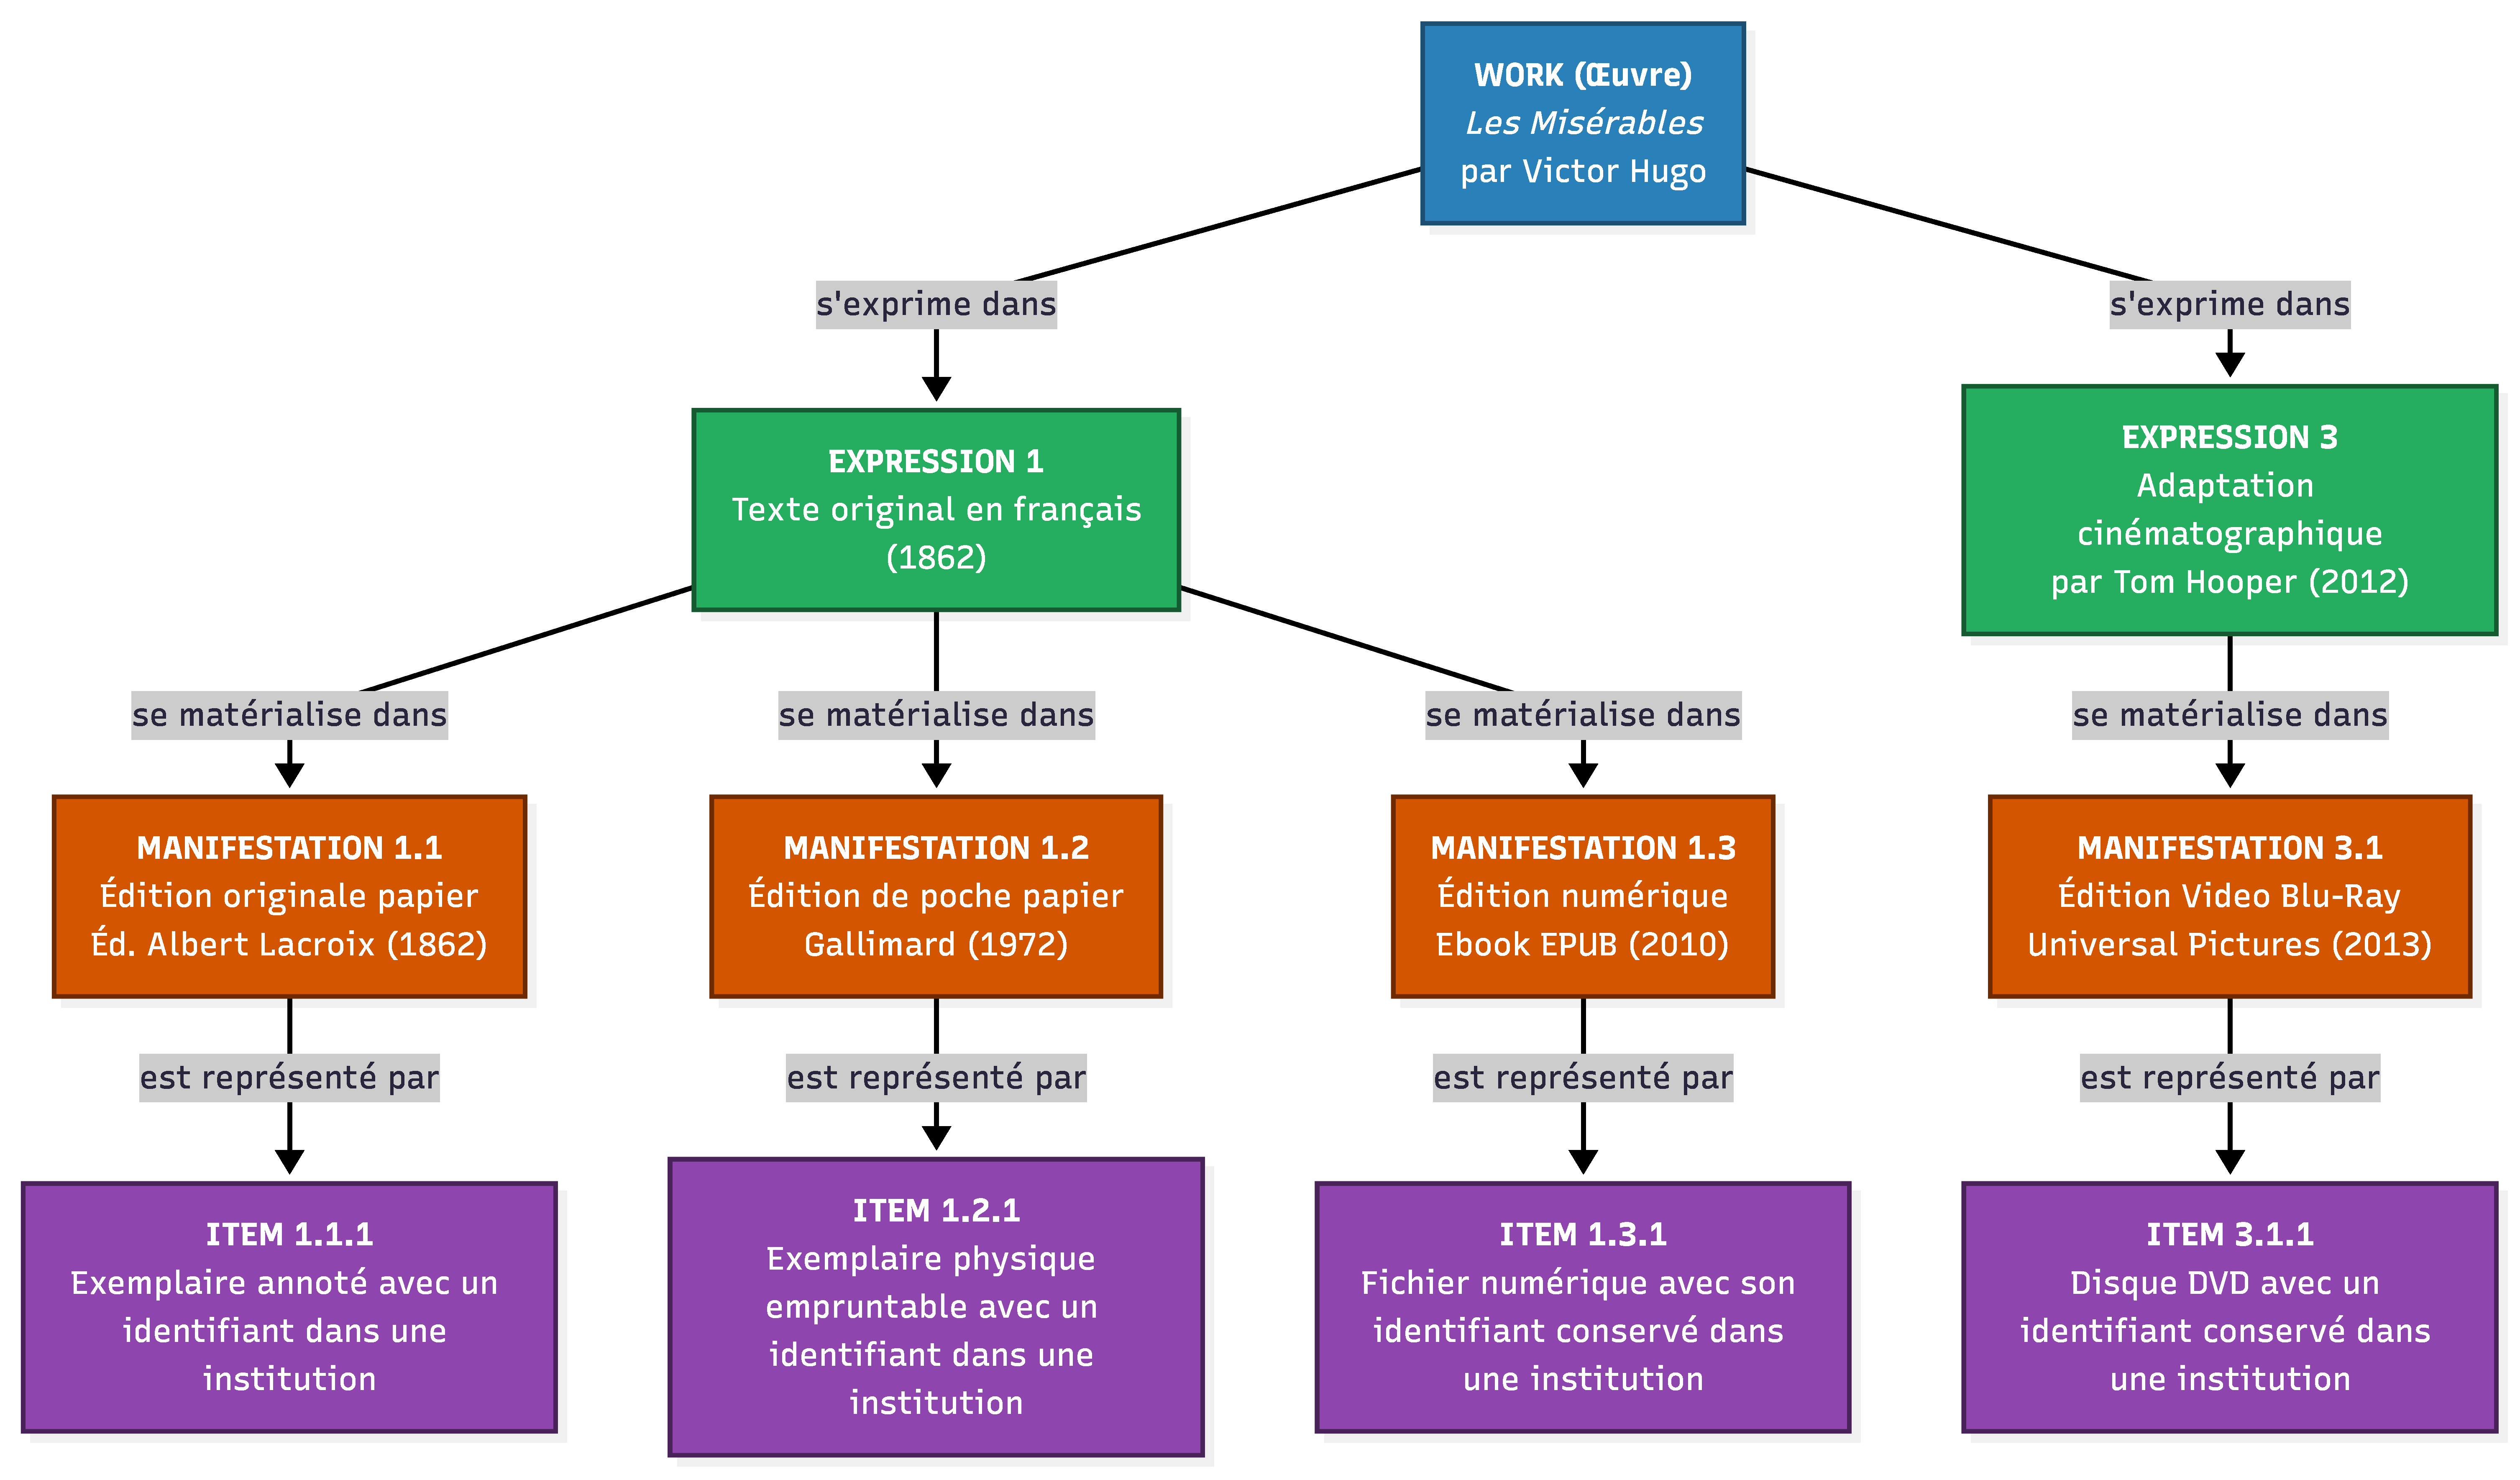
\includegraphics[width=0.9\textwidth]{./Schema/WEMI.pdf}
	\caption{Schéma d'un WEMI fictif d'une \gls{oe}.}
	\label{fig:wemiSimple_schema}
\end{figure}

Le second groupe est celui des personnes physiques et morales en lien avec chacun des niveaux \gls{WEMI} et parfois plusieurs \gls{WEMI}. 

Liée au niveau \gls{oe} elle en est la créatrice, celle qui a pensé l'idée intellectuelle. Liée au niveau \gls{exp} elle en est la réalisatrice, celle qui lui donne corps. Au niveau \gls{man}, elle en est la productrice responsable d'une forme générique qu'elle adopte. Et enfin, liée à l'\gls{it} elle en est la propriétaire. Notons que la créatrice peut aussi être réalisatrice, productrice et possesseuse au sein d'un même \gls{WEMI}. Ou alors créatrice dans un \gls{WEMI} et productrice dans un autre. Simplement, le lien avec un niveau \gls{WEMI} est toujours de même nature. \newline

Enfin, le troisième groupe est celui des éléments complémentaire au niveau \gls{oe} d'un \gls{WEMI}. on y retrouve les événements, les objets, les lieux ou les sujets qui servent donc à enrichir le niveau \gls{oe} afin de mieux l'indexer. Ce niveau peut être lié à plusieurs éléments de ce groupe et permet de créer des relations entre les \gls{oe} d'une même collection ou entre plusieurs collections. De cette manière, un utilisateur intéressé par un sujet précis peut obtenir plus de résultat à ses requêtes.\newline

De manière schématique, voilà ce que représente un \gls{WEMI} complet :

\begin{figure}[H]
	\centering
	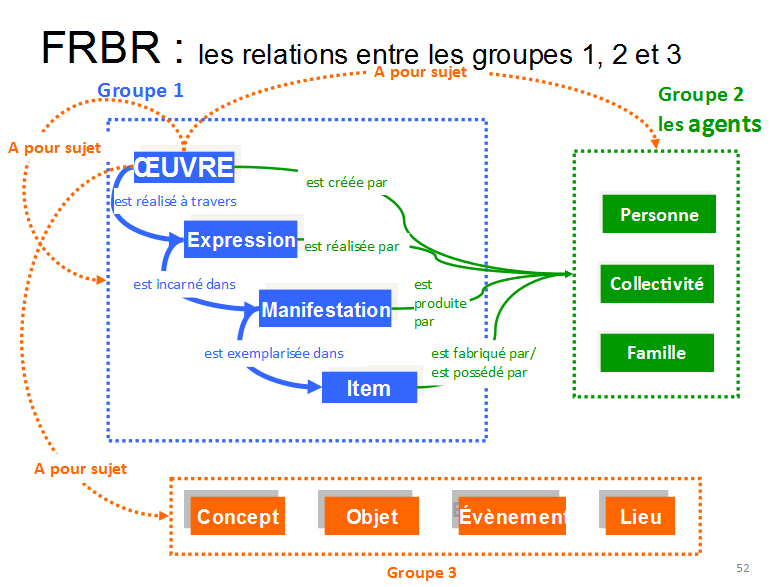
\includegraphics[width=0.7\textwidth]{./Schema/frbrComplet.png}
	\caption{Schéma de fonctionnement des liens dans un WEMI. Source : \url{https://mediadix.parisnanterre.fr/medias/fichier/catalogage-isbd-unimarc-apports-theorique-maj-2025_1736242651118-pdf}}
	\label{fig:wemiComplet_schema}
\end{figure}

Dans le cadre de l'\gls{imgani}, la \gls{FIAF} adapte ce modèle aux particularités de cette typologies. Notamment en modifiant la notion d'\gls{oe} et rajoutant celle de la \gls{vrt}.

Pour l'\gls{imgani}, l'\gls{oe} et l'\gls{exp} sont une seule et même entité.\footcite[p.21]{fairbairnManuelCatalogageImages} Ainsi, elle intègre également les circonstances de création originale de l'\gls{imgani}, des notions de temporalité, de localisation et de matérialité définies. Elle a également des relations différentes avec les personnes puisqu'elle est dotée d'une personne créatrice, mais aussi réalisatrice et productrice. Ajoutons à cela la diversité typologique importante de l'\gls{imgani} qui est incluse dans la notion d'\gls{oe} amenant à une fluctuation dans le niveau d'informations attendu.\newline

L'\gls{imgani} se caractérise également par son caractère évolutif. Outre les restaurations, elle peut être modifiée de multiples manières avant même son entrée dans une collection. Prenons l'exemple de la censure qui peut altérer la bande son, le montage ou encore l'intégrité visuelle de l'\gls{oe} impactant parfois le concept artistique exprimé. Sans constituer une \gls{oe} à part entière, elle n'est plus l'\gls{oe} originale exprimée dès la création artistique. Ainsi, la \gls{FIAF} crée une entité \gls{WEMI} unique : la \gls{vrt}.

On l'utilise dès lors qu'une modification impacte la description de l'\gls{imgani}. Que ce soit des ajouts ou des retraits de \glspl{sq}, \glspl{sc} ou \glspl{pl} ou bien des modifications dans sa production, dans les comédiens ou dans sa bande son comme par exemple un doublage.\footcite[p.23]{fairbairnManuelCatalogageImages}\newline

Ces particularités changent l'organisation du \gls{WEMI} de deux manières. D'abord sur le découpage structurel, puisque le niveau \gls{exp} disparaît laissant place à celui facultatif de la \gls{vrt}. Ensuite, sur la répartition des informations à indexer, puisque ces remaniements demandent de nouveaux points d'analyses à indexer. 

Le modèle \gls{WEMI} proposé par la \gls{FIAF} est surtout plus souple et ce décline en 4 modèles. Chacun présente une répartition différentes des informations. \footnote{Pour plus d'informations voir \cite[p.9 à 13]{fairbairnManuelCatalogageImages}} Nous n'allons pas tous les présenter ici afin de pouvoir nous attarder sur les choix effectués par SkinSoft.

\subsection{La gestion de l'\gls{imgani} dans l'application SkinSoft}

\label{S-Movies}

Dans le logiciel SkinSoft, la gestion des \gls{imgani} est réservée au module S-Movies. Nous ne reviendrons pas sur cette notion de module, déjà vue précédemment\footnote{Voir page \pageref{module}}. 

Ce qui distingue S-Movies des autres modules de la suite logicielle est sa gestion totalement transparente des niveaux \gls{WEMI}. Chaque entité \gls{WEMI} possède sa propre \gls{table}, donc ses propres données et points d'accès ce qui permet de bien cloisonner les niveaux \gls{WEMI} et de diriger l'utilisateur plus facilement entre ces derniers. La structure \gls{WEMI} adoptée est la suivante : \newpage

\begin{figure}[H]
	\centering
	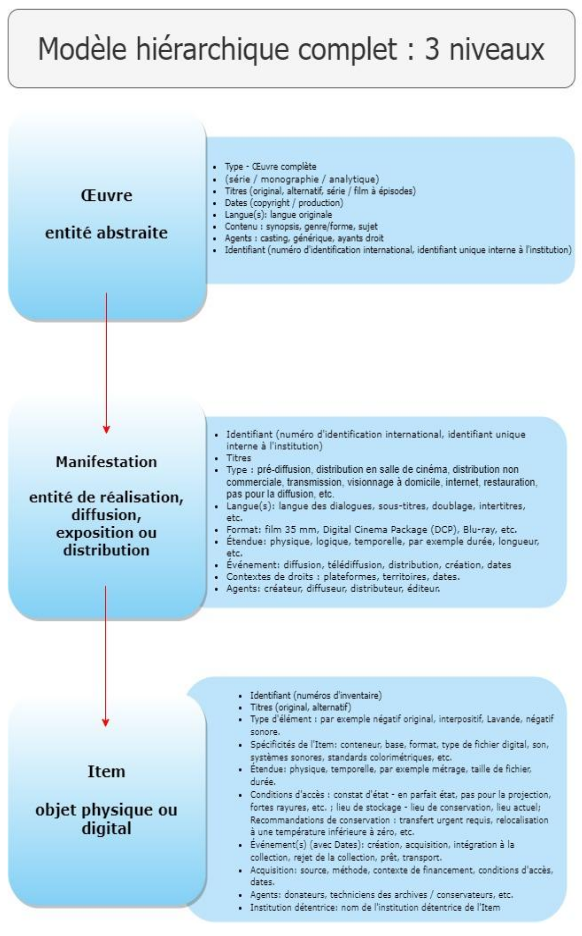
\includegraphics[width=0.8\textwidth]{./Schema/frbrSmovies.png}
	\caption{Schéma du modèle WEMI implanté dans la solution S-Movies. Source : \cite{fairbairnManuelCatalogageImages}}
	\label{fig:wemiSmovies_schema}
\end{figure}

La \gls{vrt} est considérée comme une \gls{man}. \footcite[p.23]{fairbairnManuelCatalogageImages} Ce choix vise à simplifier le parcours utilisateur en rendant son inclusion similaire à celle d'une \gls{man}, ne s'en distinguant que par un champ permettant de renseigner le type de \gls{vrt} dont il s'agit.

Les différents niveaux \gls{WEMI} sont connectés via des champ de lien créant une hiérarchie. Ils sont souples, modifiables à tout moment et multi-relationnels. Ainsi, la gestion des \glspl{imgani} reste fidèle aux principes de gestion proposés par la \gls{FIAF}\footnote{Voir \cite{fairbairnManuelCatalogageImages}}.\newline

Cette souplesse fait de S-Movies un logiciel permissif permettant à l'utilisateur d'adopter différents parcours afin d'effectuer les mêmes actions. Nous allons donc essayer de retracer un parcours utilisateur typique et privilégié, tout en énonçant les diverses possibilités s'ouvrant à lui.

L'utilisateur commence toujours par la création d'une notice \gls{oe} dans la \gls{table} dédiée, qui est également la page d'accueil de l'application. En fonction de sa configuration\footnote{Pour plus d'informations voir page \pageref{module}}, l'utilisateur peut rentrer manuellement une certaine quantité de données ce qui demande donc, en amont, une étape d'analyse afin de correctement distinguer où stocker l'information. Cette notice peut être liée à des archives, objets de musées ou des notices bibliographiques provenant des autres modules. Cela permet de créer des relations afin de circonscrire des univers cinématographiques entiers tout en gardant les spécificités de gestion de chaque objet.\newline

Ensuite, il peut créer une \gls{man} depuis la table dédiée ou une notice \gls{oe}. Si la création se fait depuis la table, elle peut être reliée à n'importe quelle \gls{oe}, et si elle est créée depuis une notice d'\gls{oe} elle y est automatiquement reliée. Peu importe la modalité, cette étape demande une analyse humaine afin de préciser la nature de la \gls{man}, notamment si c'est une \gls{vrt}. Cela demande donc une analyse effectuée au moment de la création du \gls{WEMI} et basée sur des connaissances cinématographiques. Notons qu'une \gls{man} peut être liée à plusieurs \oe{uvres}, comme les coffrets qui réunissent des \oe{uvres} différentes dans une même \gls{man}.\newline

Enfin, il peut créer un \gls{it}. Cette notice peut être créée en même temps qu'une notice d'entrée par exemple ou sous bien d'autre modalité, ce qui s'explique par le fait que c'est à ce niveau qu'on gère le \guillemet{cycle de vie} pensé par David Bearman.\footcite{ArchivesMuseumInformatics} Notons que plusieurs \gls{it} peuvent être liés à une seule \gls{man}.

\subsection{Complexité et limite de l'indexation des \glspl{imgani}}

Les \glspl{imgani} sont très riches en informations visuelles, parfois textuelle avec les crédits. Il faut donc pouvoir récupérer ces données, ce qui demandent des traitements différents puis les répartir sur les niveaux \gls{WEMI} appropriés. Dans les productions amatrices, les informations à indexer sont souvent uniquement visuelles ce qui demande d'analyser chaque \gls{oe} afin d'en extraire des mots-clés, des caractéristiques uniques, etc, ainsi que d'en déterminer le niveau \gls{WEMI} d'appartenance. 

Rajoutons également que l'indexation se complexifie avec la question de l'héritage des champs notamment pour la \gls{vrt}. En effet, une donnée portée par l'\gls{oe}, comme les comédiens, peut se retrouver invalide dans la \gls{vrt} en découlant. Cela peut créer une incohérence d'indexation et des difficultés de modifications de la donnée.\newline

\label{imganiExemple} Pour illustrer ces limites, prenons le cas d'une institution aux besoins de gestion spécifiques et utilisant S-Movies.\footnote{Pour des raisons de sécurité et de confidentialité, le nom de l'institution est anonymisé.} 

Certaines \glspl{imgani} ont été réunies sur un même support de conservations sans séparation entre les \gls{oe}. Deux problématiques en émergent : d'abord un \gls{WEMI} complexe, puisque plusieurs \glspl{oe} sont réunies en une seule \gls{man} d'où découle plusieurs \glspl{it}. De plus, le besoin de séparer matériellement dans l'application chaque bande vidéos et sonore de chaque \gls{it} afin de pouvoir les reconstituer dans des notices. 

Son schéma \gls{WEMI} est réalisable, mais toute l'étape de traitement est problématique. Il repose sur l'analyse de bobines entières, l'identification de chaque entités présentes et de leur association au segment de bobine concerné. Cependant, cela ne peut être fait que par l'humain à l'aide de logiciels de traitement externes spécialisé. De plus, il n'y a aucun crédit permettant des identifications de caractéristiques clés facilement. Après avoir segmenté les bobines en plusieurs \glspl{imgani}, il faut les analyser individuellement pour en extraire des informations clés. Ce qui peut être long, fastidieux et prompt aux erreurs humaines.\newline 

Cet exemple met en valeur les problématiques principales de l'indexation de cette typologie documentaire. SkinSoft cherche aujourd'hui à faire évoluer S-Movies pour proposer des modalités de gestions plus adaptées par le déploiement d'un outil d'indexation semi-automatisée notamment afin d'automatiser et homogénéiser les indexations. Ce serait un \textit{pipeline} basé sur l'\gls{IA} allant de l'intégration dans l'application d'une vidéo à son indexation, en passant par sa segmentation en différentes \glspl{imgani} indexées individuellement.